\documentclass[aspectratio=169]{beamer}
% \documentclass{beamer}

\usetheme{numpex}

\usepackage{tikz,pgfplots}
\usepackage{booktabs}
\usepackage[scale=2]{ccicons}



\title{A new beamer theme for NumPEx}
\subtitle{This is a subtitle}
\date{\today}
\author{Alfredo Buttari}
\institute{Institute or miscellaneous information}

\begin{document}

\maketitle

\begin{frame}[fragile]{NumPEx theme}

  The NumPEx theme is a Beamer theme with minimal visual noise
  inspired by the 

  \vspace{0.1cm}
  
  \begin{center}
    \alert{\href{https://www.info.gouv.fr/marque-de-letat}{Charte
        graphique de l'etat Français}}
  \end{center}

  \vspace{0.4cm}
  
  Enable the theme by loading

\begin{verbatim}
  \usetheme{numpex}
\end{verbatim}

  \vspace{0.4cm}

  Note, that you have to have \emph{Marianne} font and XeTeX
  installed to enjoy this wonderful typography. You can find the font
  
  \vspace{0.1cm}
  
  \begin{center}
    \alert{\href{https://www.systeme-de-design.gouv.fr/elements-d-interface/fondamentaux-de-l-identite-de-l-etat/typographie/}{here}}
  \end{center}
\end{frame}

\begin{frame}[fragile]
  \frametitle{Sections}
  Sections group slides of the same topic

\begin{verbatim}
    \section{Elements}
\end{verbatim}

  for which the NumPEx theme provides a nice progress indicator \ldots
\end{frame}

\section{Elements}

\begin{frame}{Typography}

The theme provides sensible defaults to \emph{emphasize}
text, \alert{accent} parts or show \textbf{bold} results.
\end{frame}

\begin{frame}{Lists}
  \begin{columns}[onlytextwidth]
    \column{0.5\textwidth}
      Items
      \begin{itemize}
        \item Milk \item Eggs \item Potatos
      \end{itemize}

    \column{0.5\textwidth}
      Enumerations
      \begin{enumerate}
        \item First, \item Second and \item Last.
      \end{enumerate}
  \end{columns}
\end{frame}
\begin{frame}{Descriptions}
  \begin{description}
    \item[PowerPoint] Meeh.
    \item[Beamer] Yeeeha.
  \end{description}
\end{frame}
\begin{frame}{Animation}
  \begin{itemize}[<+- | alert@+>]
    \item \alert<4>{This is\only<4>{ really} important}
    \item Now this
    \item And now this
  \end{itemize}
\end{frame}


\begin{frame}{Tables}
  \begin{table}
    \caption{Largest cities in the world (source: Wikipedia)}
    \begin{tabular}{lr}
      \toprule
      City & Population\\
      \midrule
      Mexico City & 20,116,842\\
      Shanghai & 19,210,000\\
      Peking & 15,796,450\\
      Istanbul & 14,160,467\\
      \bottomrule
    \end{tabular}
  \end{table}
\end{frame}
\begin{frame}{Blocks}

  \begin{block}{This is a block title}
    Hello
  \end{block}

  \begin{exampleblock}{This is an example block}
    Hello
  \end{exampleblock}


  
\end{frame}
\begin{frame}{Math}
  \begin{equation*}
    e = \lim_{n\to \infty} \left(1 + \frac{1}{n}\right)^n
  \end{equation*}
\end{frame}

\begin{frame}{Line plots}
\begin{center}
  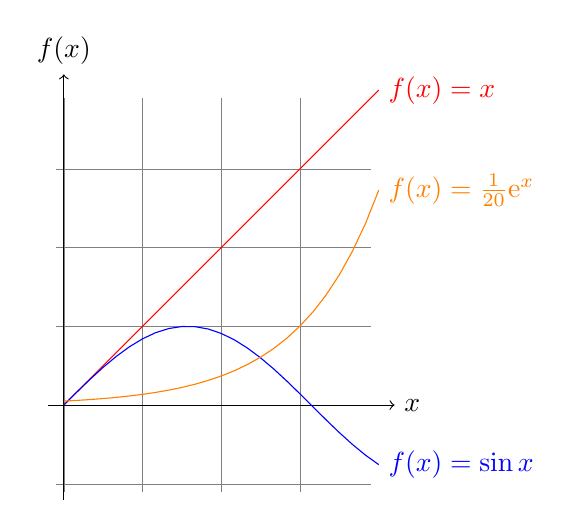
\begin{tikzpicture}[domain=0:4]
    \draw[very thin,color=gray] (-0.1,-1.1) grid (3.9,3.9);
    
    \draw[->] (-0.2,0) -- (4.2,0) node[right] {$x$};
    \draw[->] (0,-1.2) -- (0,4.2) node[above] {$f(x)$};
    
    \draw[color=red]    plot (\x,\x)             node[right] {$f(x) =x$};
    % \x r means to convert '\x' from degrees to _r_adians:
    \draw[color=blue]   plot (\x,{sin(\x r)})    node[right] {$f(x) = \sin x$};
    \draw[color=orange] plot (\x,{0.05*exp(\x)}) node[right] {$f(x) = \frac{1}{20} \mathrm e^x$};
  \end{tikzpicture}
\end{center}
% \begin{figure}
%     \begin{tikzpicture}
%       \begin{axis}[
%         mlineplot,
%         width=0.9\textwidth,
%         height=6cm,
%       ]

%         \addplot {sin(deg(x))};
%         \addplot+[samples=100] {sin(deg(2*x))};

%       \end{axis}
%     \end{tikzpicture}
%   \end{figure}
\end{frame}


\begin{frame}[fragile]{Bar charts}

  \begin{center}
\begin{tikzpicture}
\begin{axis}[
  x tick label style={
    /pgf/number format/1000 sep=},
  ylabel=Population,
  enlargelimits=0.15,
  legend style={at={(0.5,-0.15)},
    anchor=north,legend columns=-1},
  ybar,
  bar width=7pt,
  ]
  \addplot [color=nred, fill=nred!30]
  coordinates {(1930,50e6) (1940,33e6)
    (1950,40e6) (1960,50e6) (1970,70e6)};
  
  \addplot [color=nblue, fill=nblue!30]
  coordinates {(1930,38e6) (1940,42e6) 
    (1950,43e6) (1960,45e6) (1970,65e6)};
  
  \addplot [color=ngreen, fill=ngreen!30]
  coordinates {(1930,15e6) (1940,12e6) 
    (1950,13e6) (1960,25e6) (1970,35e6)};
  
  \addplot[red,sharp plot,update limits=false] 
  coordinates {(1910,4.3e7) (1990,4.3e7)} 
  node[above] at (axis cs:1950,4.3e7) {Houses};
  
  \legend{Far,Near,Here,Annot}
\end{axis}
\end{tikzpicture}  \end{center}

\end{frame}



\begin{frame}[fragile]{Code}

  I love Fortran!
  
  \vspace{0.5cm}

\begin{lstlisting}[basicstyle=\tt\scriptsize, showlines=true]
program pippo

  integer, parameter            :: m=10, n=5
  real(kind(1.d0)), allocatable :: a(:,:)

  allocate(a(m,n))      ! allocate the matrix

  call random_number(a) ! fill it up

  call do_something(a)  ! do something on it

  write(*,'("Hello world")')
  stop

end program pippo
\end{lstlisting}

\end{frame}

\section{Conclusion}

\begin{frame}{Summary}

  Get the source of this theme and the demo presentation from

  \begin{center}\url{http://somewhere}\end{center}

\end{frame}

\plain{Questions?}

\end{document}

%%% Local Variables:
%%% mode: latex
%%% TeX-master: t
%%% TeX-engine: xetex
%%% TeX-command-extra-options: "--synctex=1"
%%% End:
